% !TEX root = ../viktomas-master.tex
% pokyny
% Z uživatelského hlediska je velmi výhodné před nákupem zboží prozkoumat trh pomocí internetových srovnávačů. Zatím ovšem není snadno dostupná služba, která by uživateli umožnila vytvořit si hypotetický seznam zboží, které zvažuje koupit.

% *Vytvořte rešerši stávajících systémů zabývajících se organizací nákupních seznamů.
% *Zjistěte možnosti a strategii napojení na systémy zabývající se srovnáním a sledováním cen.
% *V souladu s touto rešerší poté analyzujte, navrhněte a implementujte webovou aplikaci, která bude umožňovat přidávat, sledovat, prioritizovat a kategorizovat zboží, zobrazovat jeho cenu a její vývoj.
% *Webovou aplikaci implementujte v jazyce Ruby ve vhodném frameworku.
% *Pro prioritizaci navrhněte a implementujte vhodné algoritmy.
% *API webové aplikace bude navrženo s ohledem na budoucí integraci s dalšími systémy (např. srovnávače cen apod.).
\chapter{Rešerše}
Tato kapitola se zabývá popisem problematiky této práce. V zadání práce je řečeno, že má být vytvořena rešerše stávajících systémů zabývajících se organizací nákupního seznamu. Tato rešerše je rozdělena na 3 kapitoly z nichž každá řeší jeden aspekt těchto seznamů.

\section{Nákupní seznamy}

\subsection{Google ShoppingList}
Webová aplikace založená na službě Google Nákupy. Podporuje jednoduché přidání zboží. U přidaných položek zobrazuje následující informace a umožňuje podle nich i řadit:
\begin{itemize}
\item Datum přidání položky
\item Nejnižší aktuální cena
\item Hodnocení ostatních uživatelů
\end{itemize}
Nákupní seznam je v základním nastavení veřejný a je možné zkopírovat na něj odkaz. Tento odkaz následně uživatel odešle komukoli, s kým chce svůj nákupní seznam sdílet. U každé položky na seznamu je možné vypnout sdílení.

Další funkčnost, kterou nabízí tento seznam je:
\begin{itemize}
\item Přidání poznámky k položce - uživateli je umožněno přidat poznámku k položce na seznamu.  Tato poznámka je následně zobrazena u položky v hlavním přehledu.
\item Odebrání položky ze seznamu
\item Zrušení sdílení - viz. předchozí odstavec
\end{itemize}

\begin{figure}[htb]
\begin{center}
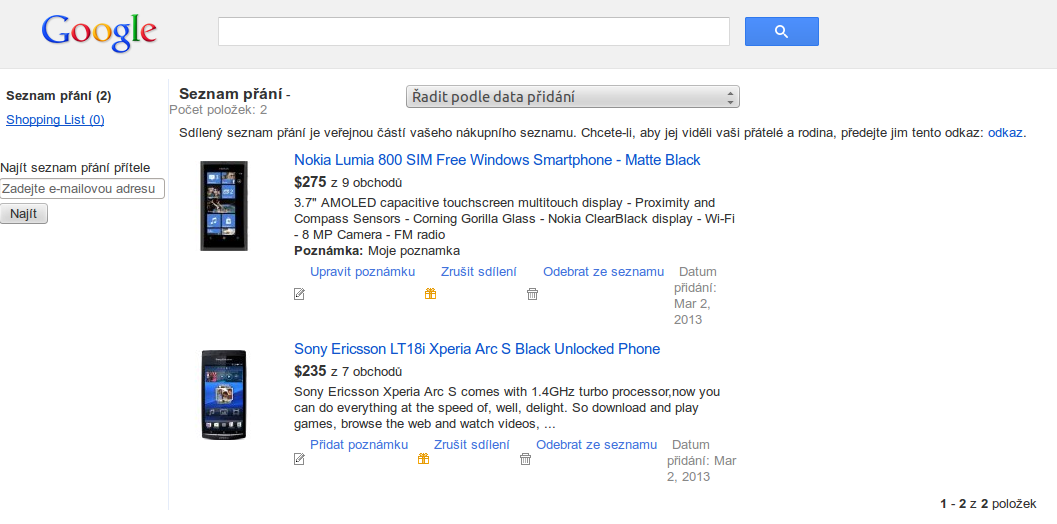
\includegraphics[width=120mm]{./pictures/google-shopping-list.png}
\caption{Google ShoppingList - základní obrazovka}
\label{fig:google-shoppinglist}
\end{center}
\end{figure}

\subsection{Amazon Wish List}
Amazon Wish List je funkcionalita poskytovaná komplementárně k internetovému obchodu Amazon.com. Služba umožňuje vytvářet a sdílet seznamy přání. Pro využívání této služby musí být uživatel přihlášen. Pokud se nepřihlášený uživatel pokusí přidat nějaký předmět do seznamu přání, je přesměrován na stránku přihlášení.

\subsubsection{Druhy přání}
Tato sekce se zabývá druhy přání ve službě Amazon Wish List. Přáním se v této službě rozumí tři věci:
\begin{itemize}
\item Produkt z internetového obchodu Amazon.com
\item Internetová stránka mimo Amazon.com
\item Nápad na přání (tzv. idea)
\end{itemize}

\paragraph{Produkt internetového obchodu Amazon.com}
Toto přání reprezentuje 1:1 produkt v internetovém obchodu Amazon.com. Toto přání vznikne tak, že přihlášený uživatel klikne na stránce produktu na tlačítko "Add To Wish List". U takovéhoto přání se ukazuje minimální možná cena, popis i obrázek.

\paragraph{Internetová stránka mimo Amazon.com}
Toto přání reprezentuje jakoukoli internetovou stránku. Přání vznikne pomocí pluginu Amazon Wish List Button. O této funkcionalitě bude pojednávat samostatná kapitola.

\paragraph{Nápad na přání}
Nápad na přání je funkcionalita, která umožní uživateli zadat nápad na přání pouze jako text (název přání). Tento nápad se uloží mezi ostatní přání. Místo obrázku přání je ovšem zobrazen obrázek nalepovacího štítku a na něm je napsáno "I Want". Nápad na přání je vidět na obrázku \ref{fig:amazon-wishlist-idea}. Každý nápad na přání má u sebe tlačítko "Top search results" které najde pro popis nápadu produkty z obchodu Amazon.com.

\begin{figure}[htb]
\begin{center}

\includegraphics[width=100mm]{./pictures/amazon-wishlist-idea.png}
\caption{Nápad na přání v Amazon Wish List}
\label{fig:amazon-wishlist-idea}
\end{center}
\end{figure}

\subsubsection{Amazon Wish List Button}
Amazon Wish List poskytuje plugin\footnote{Také zásuvný modul - software, který nepracuje samostatně, ale jako doplňkový modul jiné aplikace a rozšiřuje její funkčnost.} do všech majoritních internetových prohlížečů\cite{website:amazon:plugin}. Po nainstalovani pluginu do prohlížeče si může uživatel přidat tlačítko "Amazon Wish List Button". Po stisku tohoto tlačítka se otevře dialog. (Obrázek \ref{fig:amazon-wishlist-plugin})

\begin{figure}[htb]
\begin{center}
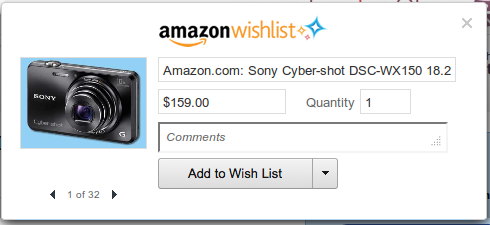
\includegraphics[width=100mm]{./pictures/amazon-wishlist-plugin.png}
\caption{Dialog zobrazeny po stisku Amazon Wish List Button}
\label{fig:amazon-wishlist-plugin}
\end{center}
\end{figure}

Přidat je možné buď produkt z obchodu Amazon. V tomto případě se načtou všechna data, která se u přání ukladájí, a není rozdíl v použití pluginu oproti stisknutí tlačítka "Add to Wish List" na stránce produktu.

Dále plugin podporuje funkci přidání přání v podobě jakékoli stránky. Tedy je možné přidat do Amazon Wish List například zboží z českého internetového obchodu. Jako obrázek k přání si uživatel může zvolit libovolý obrázek ze stránky. Jako název přání se použije titulek stránky\footnote{Obsah HTML tagu <title> ve zdrojovém kódu stránky}, popisek se k přání žádný nepřidává. Uživatel si ještě k přání muže doplnit cenu před tím než ho uloží do seznamu.

\subsection{WishList.com}
WishList.com je webová aplikace zaměřená primárně na vytváření seznamu přání. U každého seznamu podporuje sdílení a také podporuje nastavení události k seznamu a data této události. Většina seznamů má tyto hodnoty vyplněny a jsou to například seznamy přání k narozeninám, vánocům nebo seznam svatebních darů.

WishList.com neumožňuje přihlášení pomocí OpenID. Uživatel se může přihlásit pomocí svého Facebook účtu, nebo zaregistrovat klasickou metodou, kdy zadá svůj email, přihlašovací jméno a heslo.

Uživatel může vytvářet nové seznamy přání a nová přání. Při vytvoření nového seznamu zadává uživatel název seznamu, obrázek seznamu, omezení přístupu (veřejný, pouze přátelé, soukromý), popis seznamu, osobní poznámky, osobu, která si věci přeje, název a datum události. Pouze název seznamu je povinné pole. Seznam je navíc možné zabezpečit heslem.

Při přidávání přání je možné zadat prodejce předmětu, název předmětu, popis předmětu, cenu, množství, prioritu, poznámky k přání, seznam přání do kterého bude přání přidáno, příjemce přání a poté URL produktu a URL obrázku produktu. Povinným polem je pouze název předmětu.

Vytvořený seznam je možné sdílet pomocí URL. Pokud si seznam prohlíží jiný uživatel než ten, který jej vytvořil, může si tento uživatel zarezervovat přání, což znamená že koupí předmět a dá jej uživateli, který si jej přál.

Seznam přání i jednotlivá přání je možné sdílet s ostatními uživateli pomocí tlačitka "Share this WishList" resp "Share this Wish". Sdílení j e možné pomocí služeb Facebook, Myspace, Google, Twitter, Email a dalších 300+. Na sdílení je pravděpodobně použit nějaký plugin.

Přehled přání je vidět na obrázku \ref{fig:wishlist-wishlist}

\begin{figure}[htb]
\begin{center}
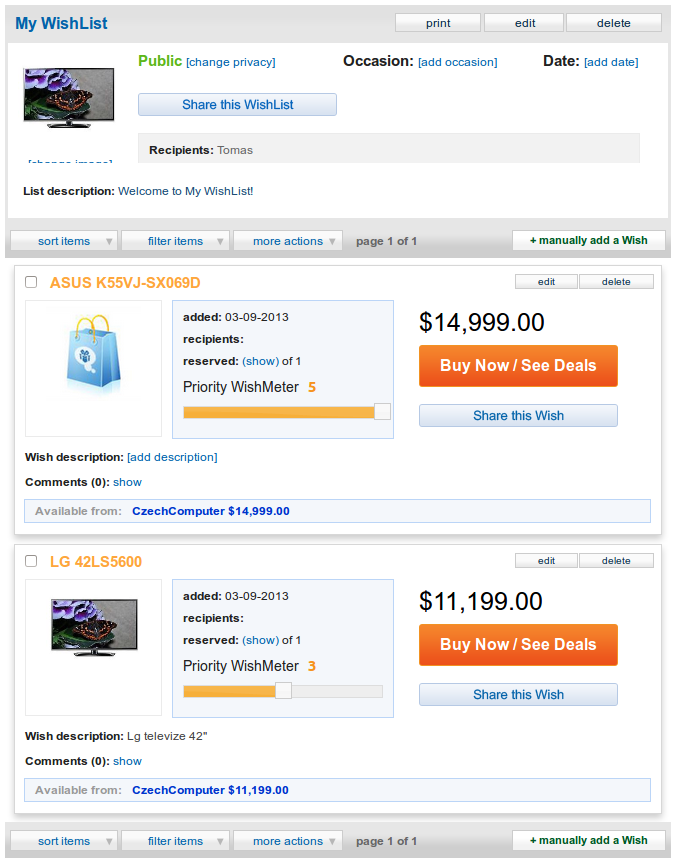
\includegraphics[width=100mm]{./pictures/wishlist-wishlist.png}
\caption{Hlavní přehled přání na stránce WishList.com}
\label{fig:wishlist-wishlist}
\end{center}
\end{figure}

\section{Srovnávače cen}
Tato kapitola poskytuje rešerši produktů známých jako srovnávače cen. Cílem těchto produktů je poskytnout uživateli širší rozhled na trh. Tyto produkty umožňují u jednoho druhu zboží (např. Televizor) srovnat jeho cenu v několika obchodech. V rešerši jsou zpracovány jako potencionální zdroje dat pro nákupní seznam.

\subsection{Standartní funkce všech srovnávačů}
V této sekci jsou popsány 3 základní funkce, které podporují všechny srovnávače cen.

\subsubsection{Vyhledávání}
Každý ze zmíňených vyhledávačů podporuje fultextové vyhledávání zboží. Dále umožňují srovnávače vyhledávání po kategoriích a/nebo filtrování parametrů zboží.

\subsubsection{Srovnávání cen}
Každý z vyhledávačů podporuje srovnání cen u zobží. U každého zboží je schopný zobrazit minimální cenu a také seznam všech obchodů s tímto zbožím a k nim přiřazenou částku, za jakou daný obchod zboží nabízí.

K této funkcionalitě zároveň patří graf historie cen. V grafu historie cen uživatel může sledovat vývoj ceny zboží a třeba odhadnout, jak se bude vyvíjet dál.

\subsubsection{Uživatelská zpětná vazba}
Touto funkčností se rozumí uživatelské hodnocení produktů a obchodů. Hodnocení většinou probíhá na principu jedné až pěti hvězdiček, případně shrnutí kladů a záporů.

\subsection{Heureka}
Interaktivní nákupní rádce Heureka.cz byl založen společností Miton v roce 2007, kdy ihned zaujmul zajímavým nápadem zkombinování mnoha užitečných možností do jednoho celku. Následně rozšiřuje svou působnost i na Slovensko a zakládá slovenskou verzi Heureka.sk (založena v r. 2008). \cite{website:wiki:heureka}

\subsubsection{Funkčnost nad rámec základní funkčnosti}
Další důležitou fukčností je hlídač ceny. Přihlášenému uživateli je umožněno na zboží nastavit hlídače ceny a poté co cena v nejlevnějším obchodě klesne pod zadanou částku, uživatel dostane email s upozorněním.

\begin{itemize}
\item Záruka vrácení peněz u některých obchodů
\item Varování před obhody, které nedodržují své obchodní podmínky
\item Sledovaní slev a novinek na trhu
\end{itemize}
\subsection{Zboží.cz}
Zboží.cz je satelitní web společnosti Seznam.cz
\footnote{Satelitní web je rozšířená a propracovanější forma tzv. microsite (jinak také minisite či weblet), jde o speciální samostatný web plnící funkce, které se na hlavní webovou prezentaci nehodí, nebo s ní dokonce nesouvisejí.}
. 

%\section{NextTag}
% \section{WunderList}

\subsection{PriceGrabber}
PriceGrabber je služba pro srovnávání cen. Jejími partnery je více než 13000 prodejců. Poskytuje volně informace o milionech produktů ve více než 25 kategoriích. Společnost také slouží jako datový zdroj pro další prodejní služby jako AOL Shopping, Bing Shopping aj. \cite{website:wiki:pricegrabber}

Price grabber byl první srovnávač, který zahrnul informace o daních a poplatcích za přepravu do srovnávání. \cite{website:wiki:pricegrabber}